\documentclass[twoside,twocolumn]{article}
    \usepackage[a4paper, left=2cm, right=2cm]{geometry} % A4 paper size and thin margins
    \usepackage[sc]{mathpazo} % Use the Palatino font
    \usepackage[T1]{fontenc} % Use 8-bit encoding that has 256 glyphs
    \usepackage{microtype} % Slightly tweak font spacing for aesthetics
    \usepackage[english]{babel} % Language hyphenation and typographical rules
    \usepackage{booktabs} % Horizontal rules in tables
    \usepackage{enumitem} % Customized lists
    \usepackage[table,xcdraw]{xcolor}
    \usepackage[utf8]{inputenc} % Required for inputting international characters
    \usepackage{parskip}
    \usepackage{graphicx}
    \usepackage{hyperref}
    \usepackage{pdfpages}
    \usepackage{amsmath}
    \usepackage{esvect}
    \usepackage{listings}
    \usepackage[title]{appendix}
    \hypersetup{
        colorlinks=true,
        linkcolor=blue,
        filecolor=magenta,      
        urlcolor=cyan,
    }
    \urlstyle{same}
    \setlength{\parindent}{18pt}
    \setlist[itemize]{noitemsep} % Make itemize lists more compact
    \makeatletter
    \newcommand*{\rom}[1]{\expandafter\@slowromancap\romannumeral #1@}
    \g@addto@macro{\UrlBreaks}{\UrlOrds}
    \makeatother

    \title{\LARGE \bf
    Background Subtraction in Video Streams
    }
    
    \author{ \parbox{3 in}{\centering Chongyi Xu \\
             University of Washington\\
             AMATH 482/582 Winter Quarter 2018\\
             {\tt\small chongyix@uw.edu}}
    }

    \begin{document}
    \maketitle

    %----------------------------------------------------------------------------------------
    %	ARTICLE CONTENTS
    %----------------------------------------------------------------------------------------
    \begin{abstract}

    For this project, we will use Dynamic Mode Decomposition method to separate the foreground object from the background 
    object. Three different videos will be imported into Matlab and a proper Dynamic Mode Decomposition reconstruction will produce 
    Low-Rank DMD and Sparse DMD. The Low-Rank DMD will be considered to be the background video and the Sparse DMD will be 
    foreground video. As the results, the reconstruction for the first video goes pretty well.
        
    \end{abstract}

    \linespread{1.05} % Line spacing - Palatino needs more space between lines
    %------------------------------------------------
    \section{Introduction and Overview}
    \subsection{Introduction}
    Dynamic mode decomposition (DMD) is a dimensional reduction algorithm developed by Peter Schmid in 2008. Given a time series of 
    data, DMD computes a set of modes each of which is associated with a fixed oscillation frequency and decay/growth rate. 
    For linear systems in particular, these modes and frequencies are analogous to the normal modes of the system, but more 
    generally, they are approximations of the modes and eigenvalues of the composition operator (also called the Koopman 
    operator). Due to the intrinsic temporal behaviors associated with each mode, DMD differs from dimensional reduction
    methods such as principal component analysis, which computes orthogonal modes that lack predetermined temporal behaviors. 
    Because its modes are not orthogonal, DMD-based representations can be less parsimonious than those generated by PCA. 
    However, they can also be more physically meaningful because each mode is associated with a damped (or driven) sinusoidal 
    behavior in time.

    %------------------------------------------------
    \subsection{Overview}
    There will be three videos to reconstruct in this project. The three videos have been uploaded into 
    \href{https://drive.google.com/open?id=1NQpCD_8bFmLH0jHF4fFBumEW4RrjgOjm}{Google Drive}. 
    \begin{itemize}
        \item An umbrella moving vertically and horizontally in the front of a wall
        \item An umbrella moving vertically and horizontally in the front of lighting screens
        \item Cars going across a bridge under sunlight.
    \end{itemize}
    For each of the video, I will first reconstruct the video using Dynamic Mode Decomposition and find out the low-rank part 
    as well as sparse part. Theoretically, the low-rank part will be background.


    %------------------------------------------------
    \section{Theoretical Background}
    \subsection{Dynamic Mode Decomposition}
    Dynamic Mode Decomposition is used to generate a dynamic model from the measurements data only. Considering we have a data 
    matrix $\mathbb{X}_{data} \in \mathbb{R}^{n * m}$. Our goal is to build a linear fit model for the dynamic system 
    $\frac{d\mathbf{x}}{dt} = A\mathbf{x}$. So we first need to divide the data matrix $\mathbb{X}$ into two matrix.
    \begin{align*}
        \mathbb{X}_{data} &= [x_1\ x_2\ x_3\ \dots x_m] \\
        \mathbb{X} &= [x_1\ x_2\ x_3\ \dots x_{m - 1}] \\ 
        \mathbb{X^\prime} &= [x_2\ x_3\ x_4\ \dots x_{m}]
    \end{align*}
    Then we want $\mathbb{X^\prime} = A\mathbb{X}$. So $A = \mathbb{X^\prime} \mathbb{X}^{+}$, where $\mathbb{X}^{+}$ is the pseudo
    inverse of matrix $\mathbb{X}$. Then, take the SVD of $\mathbb{X}_{data}$ and get $U,\ \Sigma,\ V^*$. However, since the data 
    matrix is always too large such that the computation process becomes expensive, we want to truncate the rank to $r$ for cost-less
    computation runtime. Therefore, we take the first $r$ ranks to get $U_r,\ \Sigma_r,\ V^*_r$. Then we have
    \begin{align*}
        \widetilde{A} &= U^* A U \\ 
                      &= U^* \mathbb{X^\prime} \mathbb{X}^{+} U \\
                      &= U^* \mathbb{X^\prime} V \Sigma^{-1} U^* U \\
                      &= U^* \mathbb{X^\prime} V \Sigma^{-1}
    \end{align*} 
    In order to get the linear fitting model $\frac{d\mathbf{x}}{dt} = A\mathbf{x}$, we hav our guess solution to be
    $\mathbf{x} = \mathbf{v}e^{\lambda t}$. Back to matrix size we have our solution as
    \begin{equation*}
        \widetilde{A}\Omega = \Lambda \Omega
    \end{equation*}
    where $\Omega = [eigenvectors]$ and $\Lambda =   
                                                    \begin{bmatrix}
                                                        \lambda_{1} & & \\
                                                        & \ddots & \\
                                                        & & \lambda_{r}
                                                    \end{bmatrix}$
    After having the low-rank eigenvalues and eigenvectors, we should get back to high ranks to get the solution. The DMD modes
    are defined to be 
    \begin{equation*}
        \Phi = \mathbb{X^\prime}V\Sigma^{-1}\Omega
    \end{equation*}
    And the solution we are looking for is 
    \begin{align*}
        \mathbf{X}  &= \Phi e^{\Lambda t}b \\ 
                    &= \sum_{k=1}^{r} \phi_k e^{\omega_k t}b_k
    \end{align*}
    And after we get our $\mathbf{X}_{DMD}$ as DMD reconstruction, we are looking for $p \in{1, 2, \dots r}$ satisfies
    $|| \omega_p || \approx 0$ and that any other $k \neq p$ has $|| \omega_k ||$ bounded away from zeros. Thus we have
    \begin{equation*}
        \mathbf{X}_{DMD} = \sum_{k\neq p} \phi_k e^{\omega_k t}b_k + \phi_p e^{\omega_p t}b_p 
    \end{equation*}
    where the first part is the foreground video and the second part is the background video.


    \section{Algorithm Implementation and Development}
    \subsection{General Procedure}
    \begin{itemize}
        \item Load the video files and convert the video from RGB to gray.
        \item Victories the videos and make the data matrix to have each row containing the value of the pixel and each column
        containing the time (frame), $\mathbf{X}$.
        \item Get $\mathbb{X}$ and $\mathbb{X^\prime}$ from the data matrix. And SVD $\mathbb{X}$.
        \item Perform Dynamic Mode Decomposition on the matrix.
        \item Find the index of the $\omega_p$ that satisfies the conditions introduced in the theoretical background.
        \item Construct $\mathbf{X}_{DMD}^{Low-Rank}$ and $\mathbf{X}_{DMD}^{Sparse}$.
        \item Subs tract $\mathbf{X}_{DMD}^{Low-Rank}$ from the data matrix $\mathbf{X}$
        \item Store the indices with negative values in the rest matrix $\mathbf{X}_{DMD}^{Sparse}$ and add those back to
        $\mathbf{X}_{DMD}^{Low-Rank}$.
        \item Get the $\mathbf{X}_{DMD}^{Sparse}$ again by subtracting $\mathbf{X}_{DMD}^{Low-Rank}$ from the data matrix 
        $\mathbf{X}$.
    \end{itemize}
    %------------------------------------------------

    \section{Computational Results}
    \subsection{Video 1}
    \begin{figure}[h]
        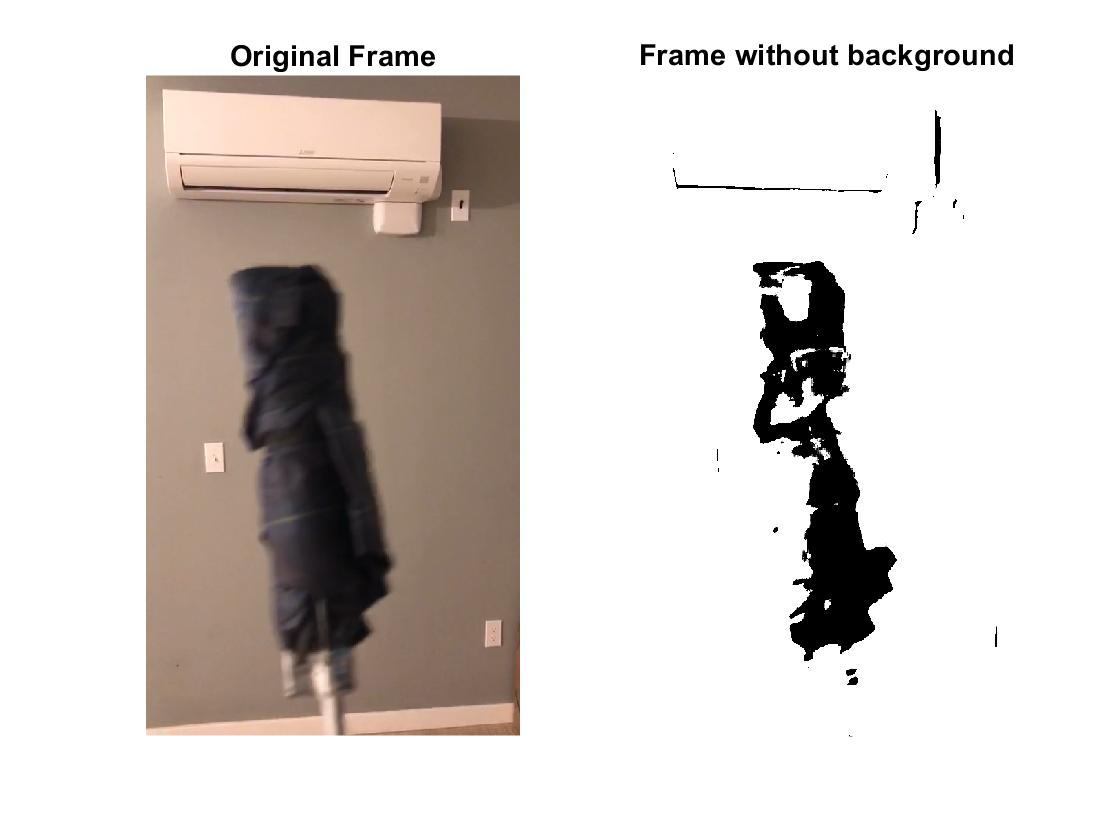
\includegraphics[width = 0.45\textwidth]{1.jpg}
        \caption{Comparison For Video 1}
        \label{fig:1}
    \end{figure}
    For the first video, we can see that at this frame, the background has been successfully removed.

    \subsection{Video 2}
    \begin{figure}[h]
        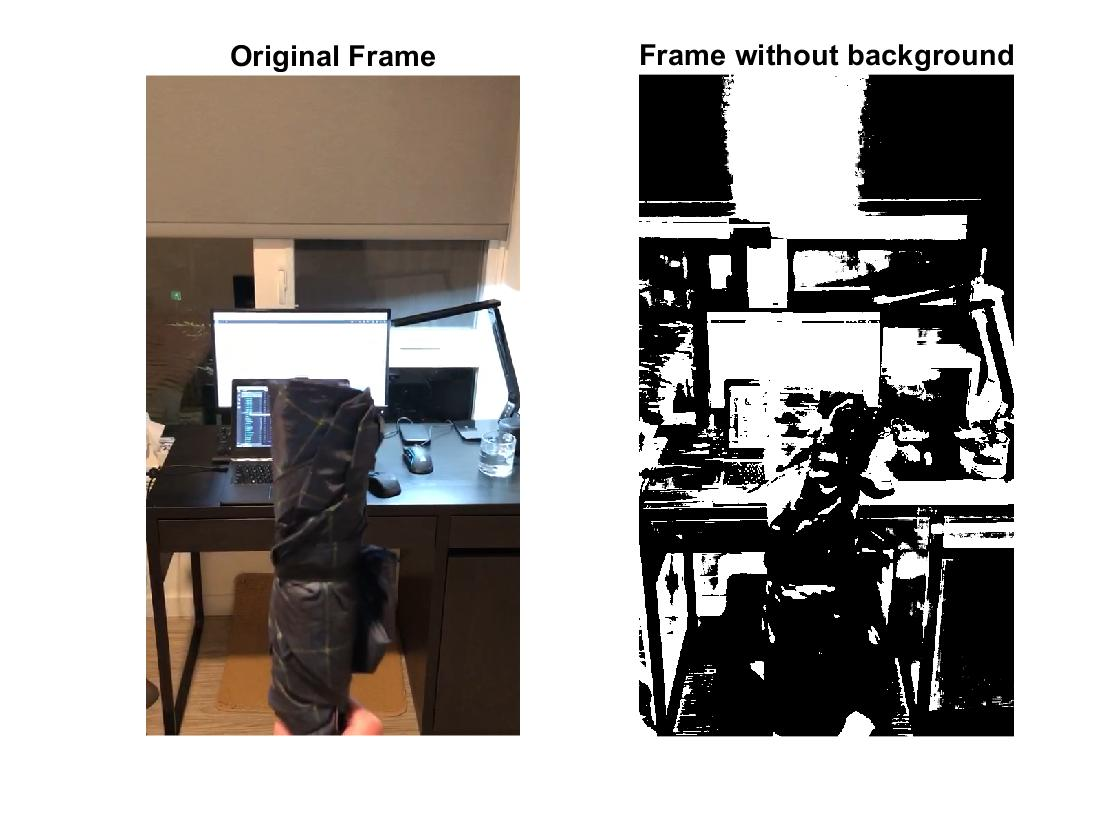
\includegraphics[width = 0.45\textwidth]{2.jpg}
        \caption{Comparison For Video 2}
        \label{fig:2}
    \end{figure}
    For the second video, the removal is not as ideal as the first video but still successfully removed
    most of the background view in the frame.

    \subsection{Video 3}
    \begin{figure}[h]
        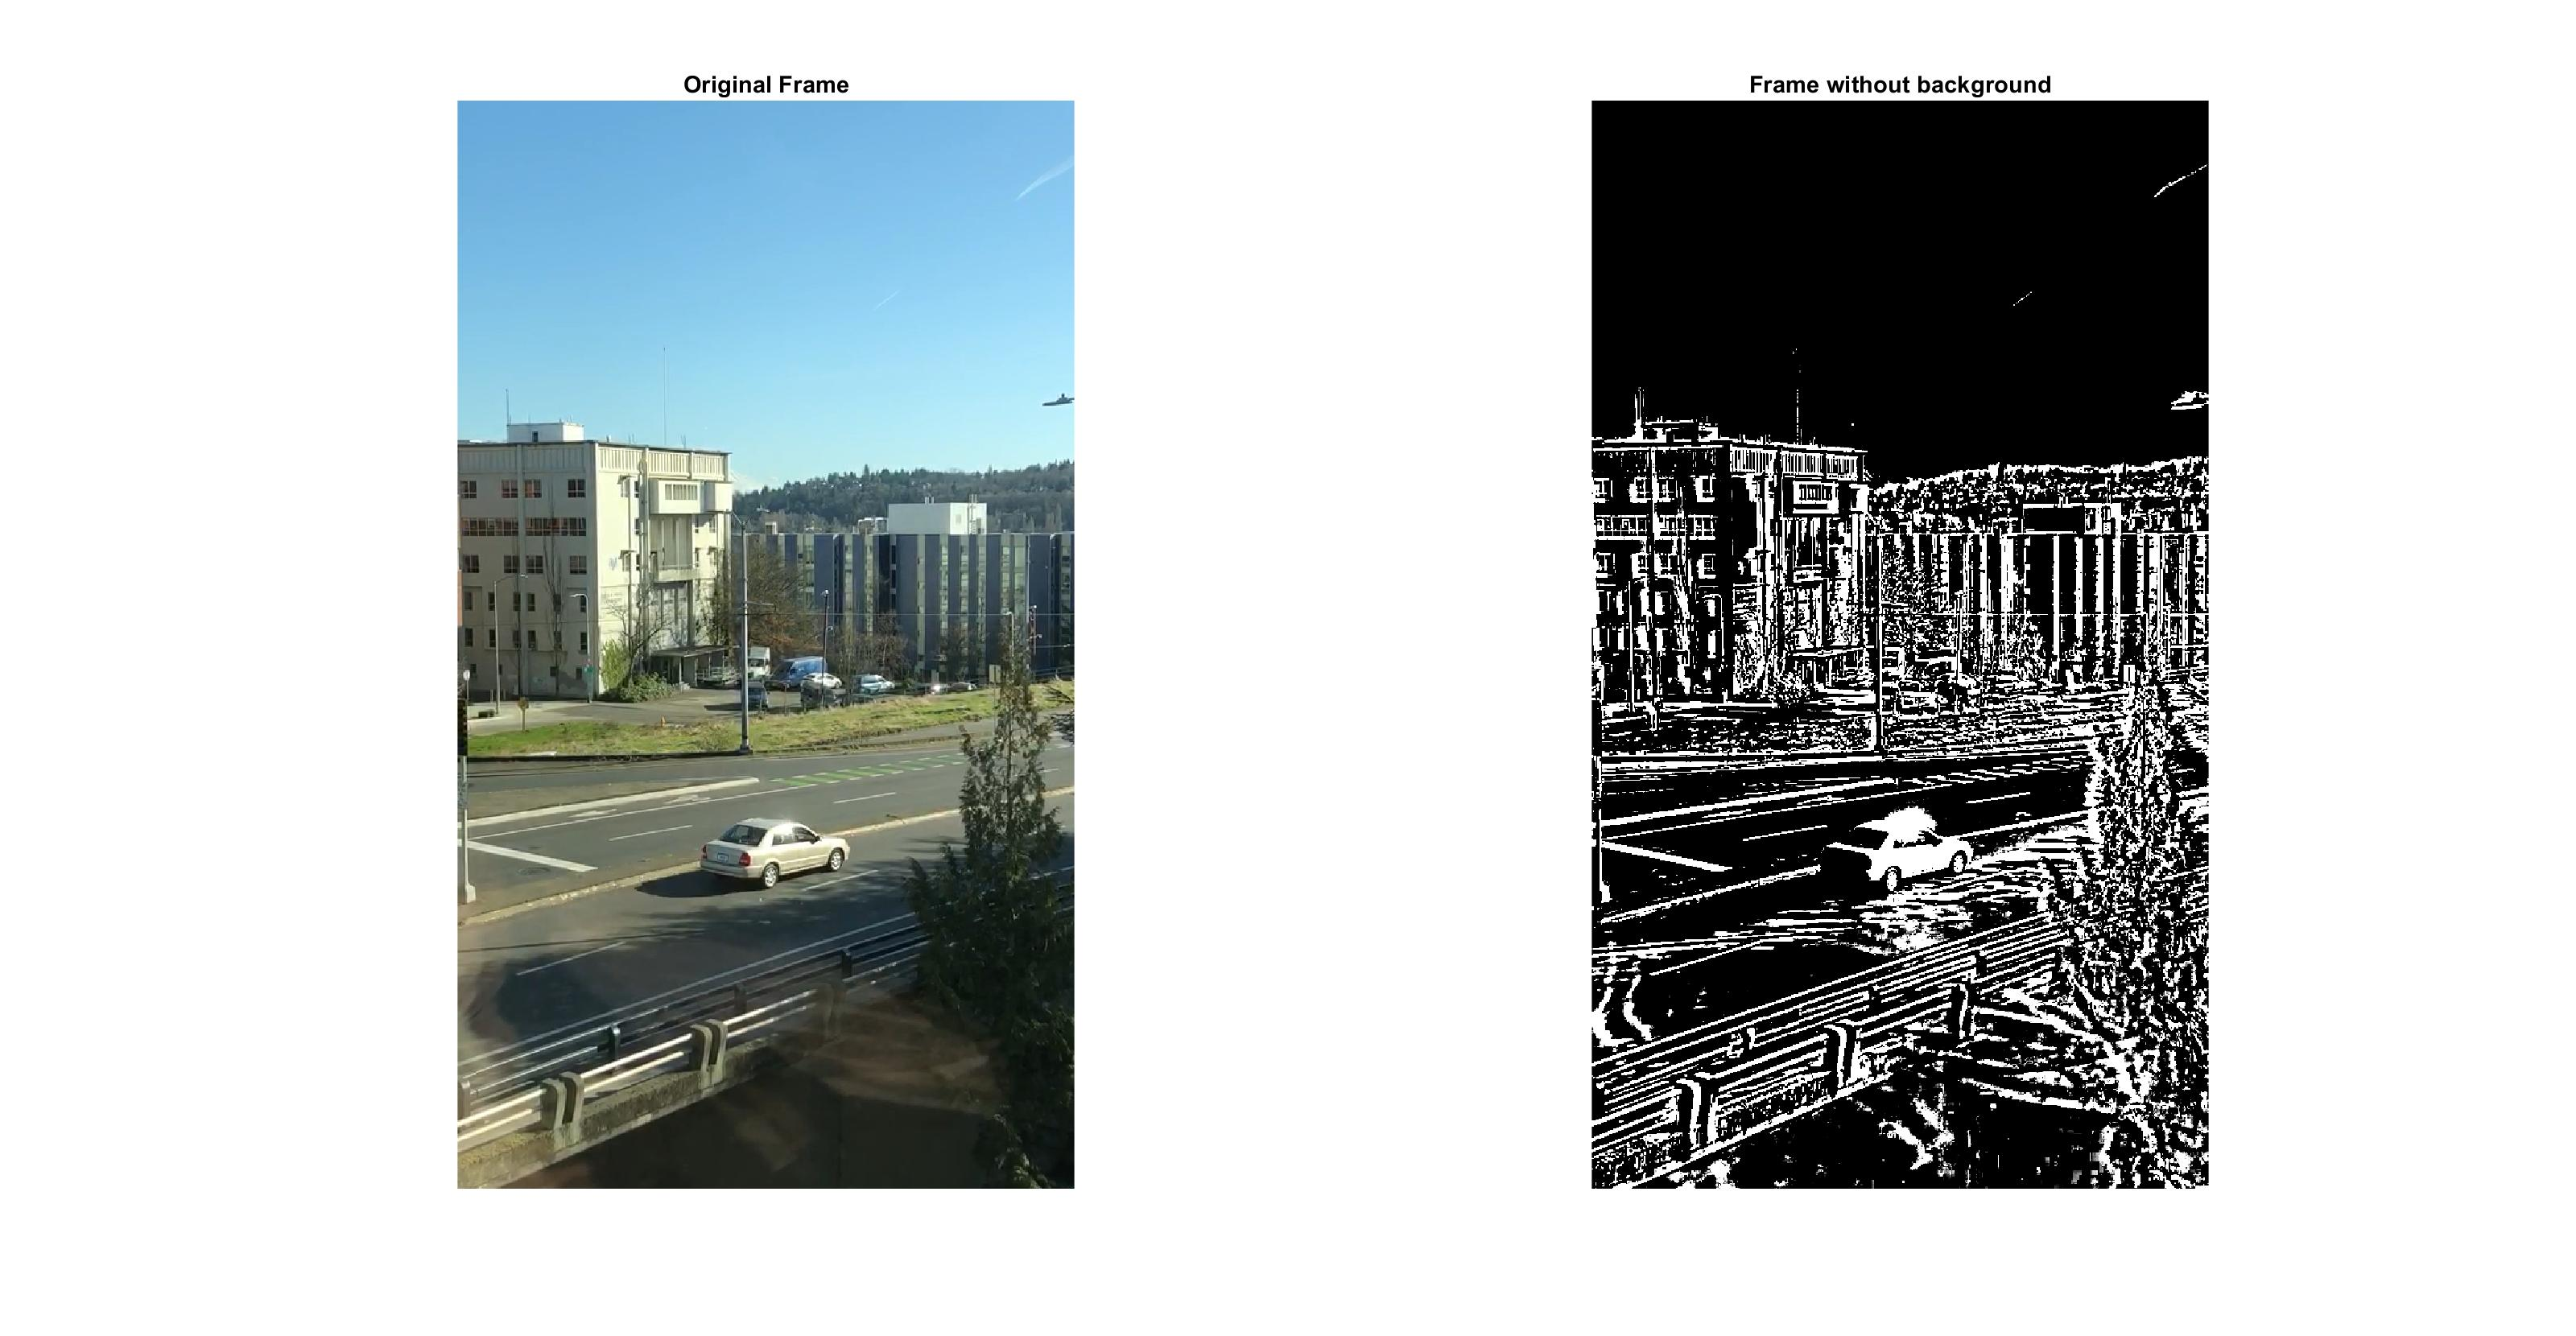
\includegraphics[width = 0.45\textwidth]{3.jpg}
        \caption{Comparison For Video 2}
        \label{fig:3}
    \end{figure}
    And for the last video, the removal does not work pretty well, which is reasonable since the video frame
    is too complicated with too many elements.
    
    \section{Summary and Conclusion}
    Dynamic Mode Decomposition is super powerful. It is possible to build a model to the dynamic system and 
    approximate the future behavior. Using DMD to process the similar application as background substraction
    to video stream as we did in this project, it might be important to have a "simple" video as possible.
    %----------------------------------------------------------------------------------------
    %	APPENDIX
    %----------------------------------------------------------------------------------------

    \mbox{~}
    \clearpage
    \begin{appendices}
    \setboolean{@twoside}{false}
    \setboolean{@twocolumn}{false}
        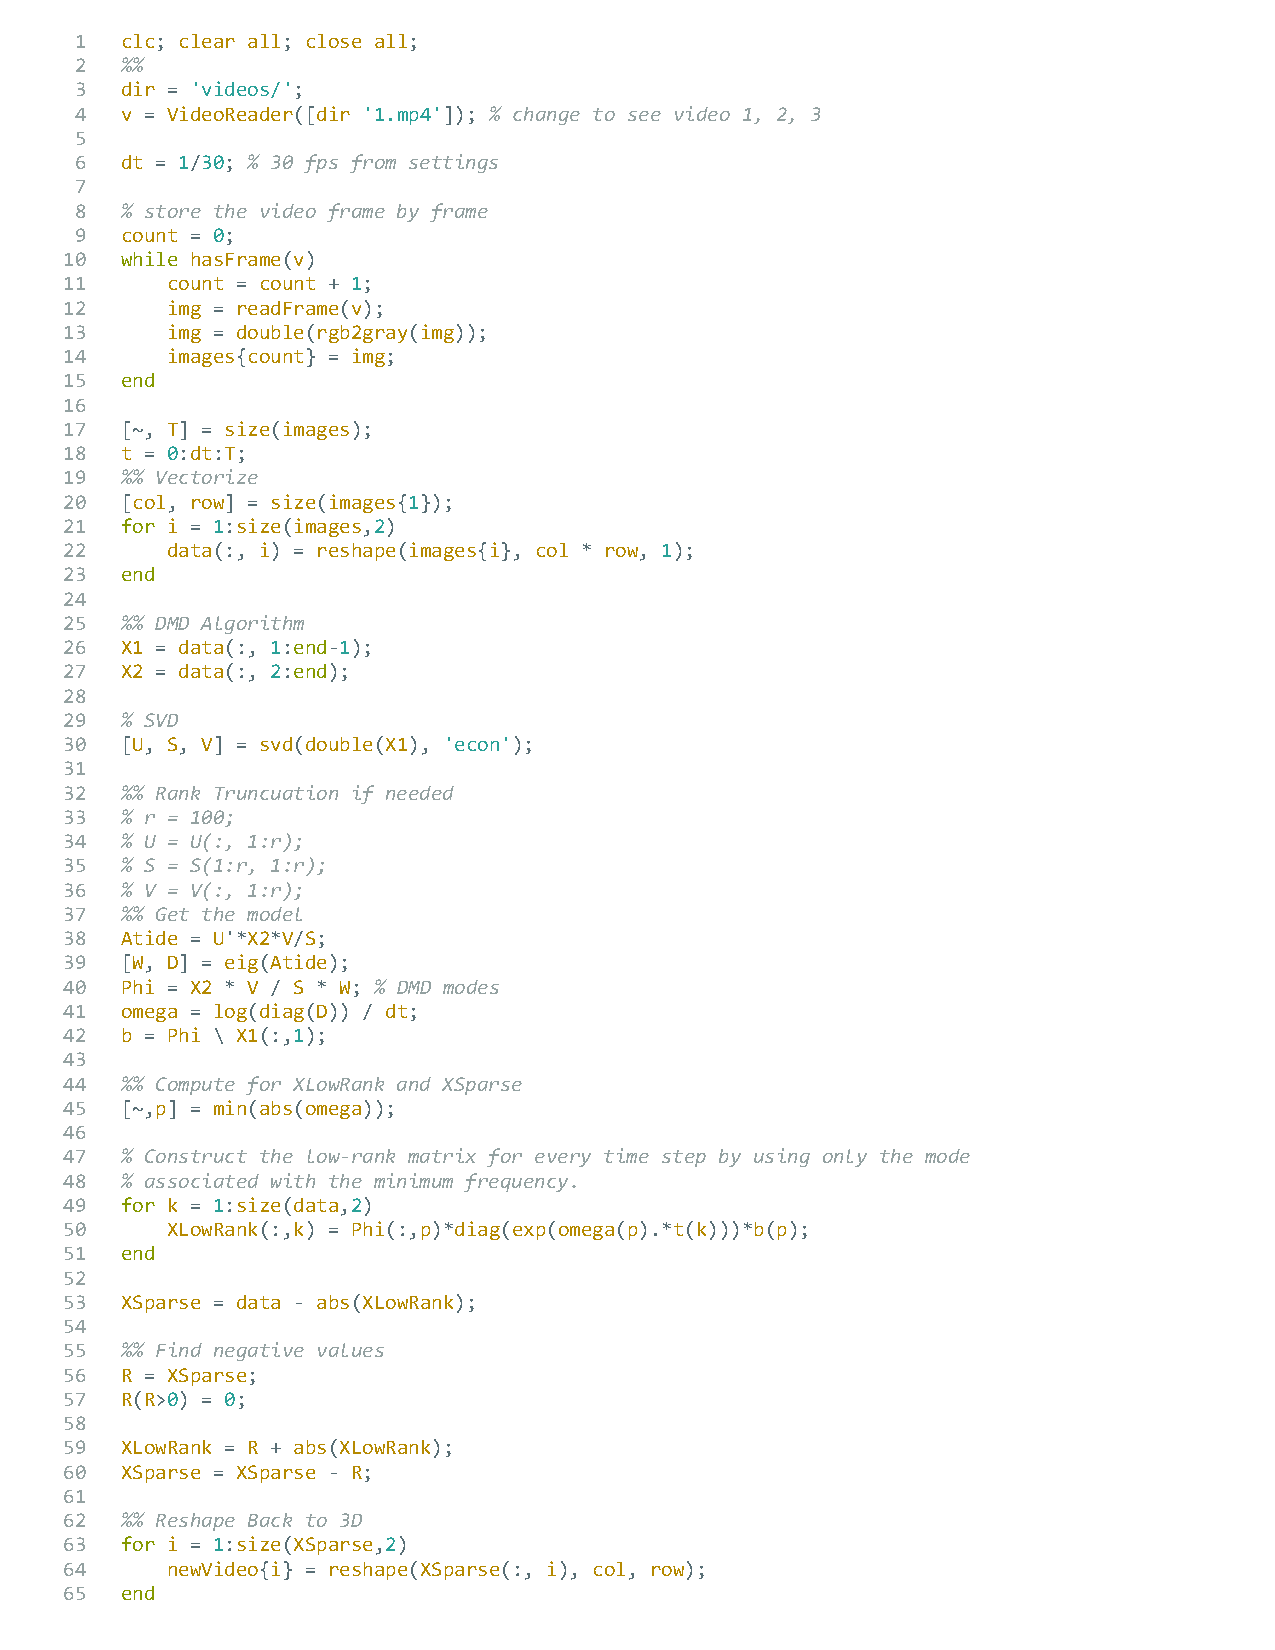
\includepdf[pages=-]{appendix.pdf}
    \end{appendices}

\end{document}